\subsection*{Positive Clipper Circuit}

% Sine Wave

\begin{figure}[H]
  \centering

  \begin{subfigure}[b]{0.49\textwidth}
    \centering
    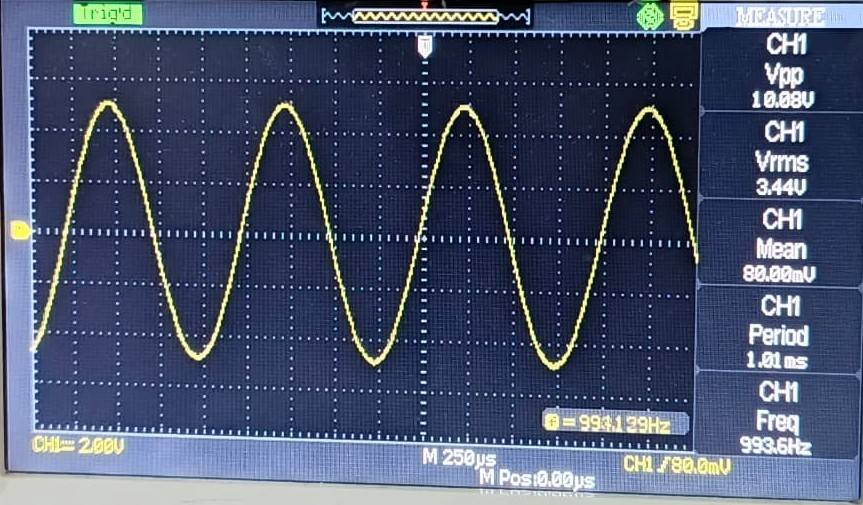
\includegraphics[width=\textwidth, keepaspectratio]{lab-05/assets/clipper/input-sine-wave.jpeg}
    \caption{ }
  \end{subfigure}
  \hfill
  \begin{subfigure}[b]{0.49\textwidth}
    \centering
    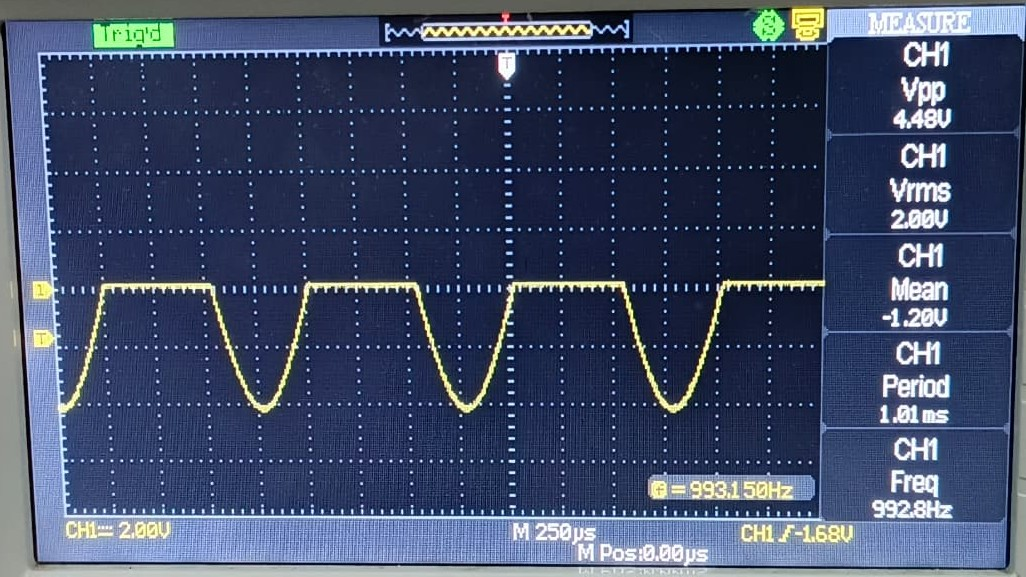
\includegraphics[width=\textwidth, keepaspectratio]{lab-05/assets/clipper/postive-output-sine-wave.jpeg}
    \caption{ }
  \end{subfigure}

  \caption{(a) Input and (b) Output Wave Shape for Positive Clipper (Sine Waves)}
  \label{fig:lab05_positive_sine}
\end{figure}

% Square Wave

\begin{figure}[H]
  \centering

  \begin{subfigure}[b]{0.49\textwidth}
    \centering
    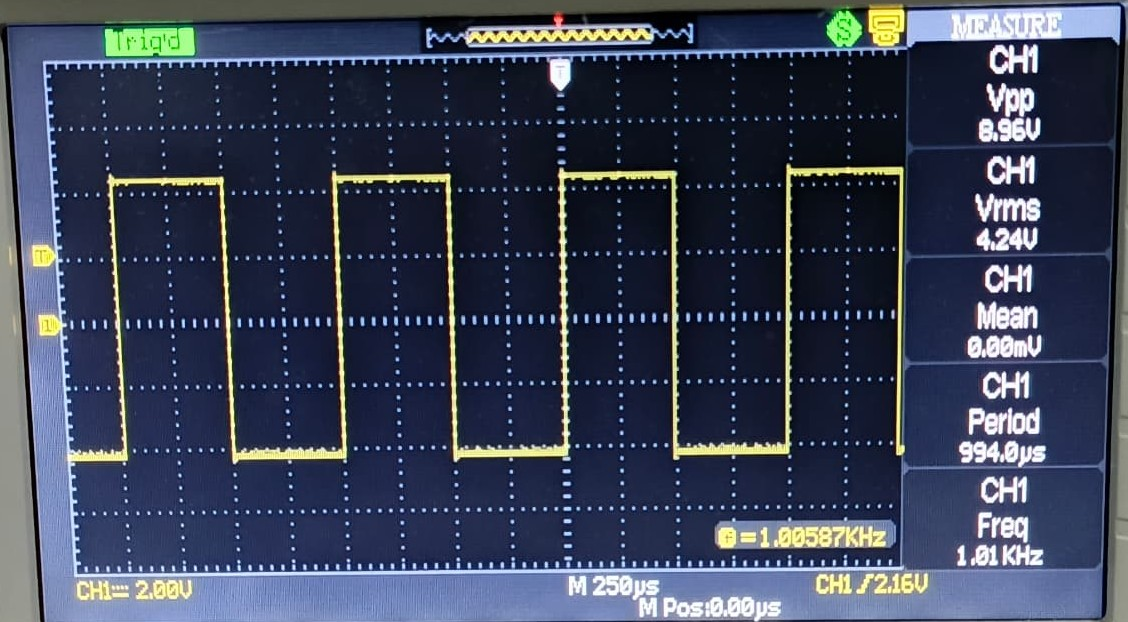
\includegraphics[width=\textwidth, keepaspectratio]{lab-05/assets/clipper/input-sqaure-wave.jpeg}
    \caption{ }
  \end{subfigure}
  \hfill
  \begin{subfigure}[b]{0.49\textwidth}
    \centering
    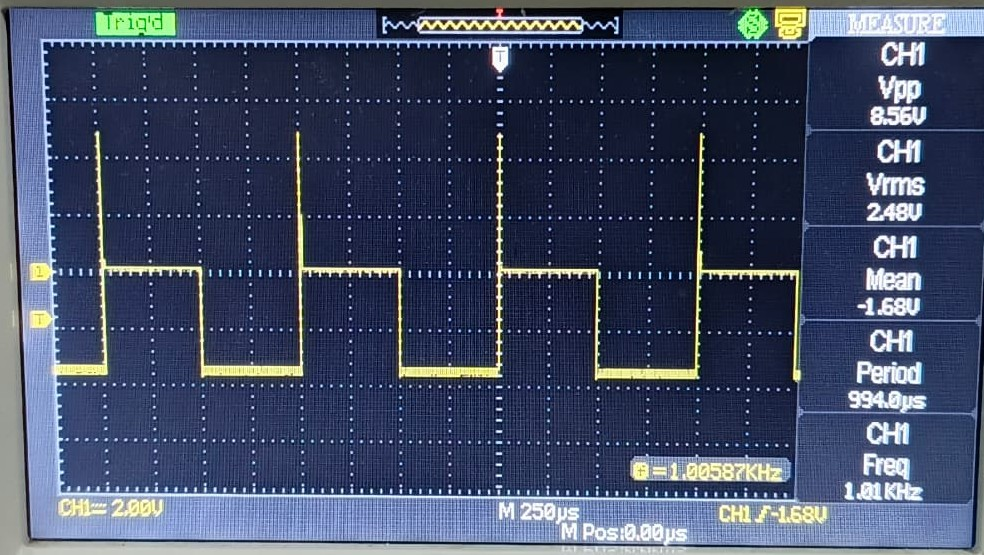
\includegraphics[width=\textwidth, keepaspectratio]{lab-05/assets/clipper/postive-output-square-wave.jpeg}
    \caption{ }
  \end{subfigure}

  \caption{(a) Input and (b) Output Wave Shape for Positive Clipper (Sqaure Waves)}
  \label{fig:lab05_positive_square}
\end{figure}

% Triangular Wave

\begin{figure}[H]
  \centering

  \begin{subfigure}[b]{0.49\textwidth}
    \centering
    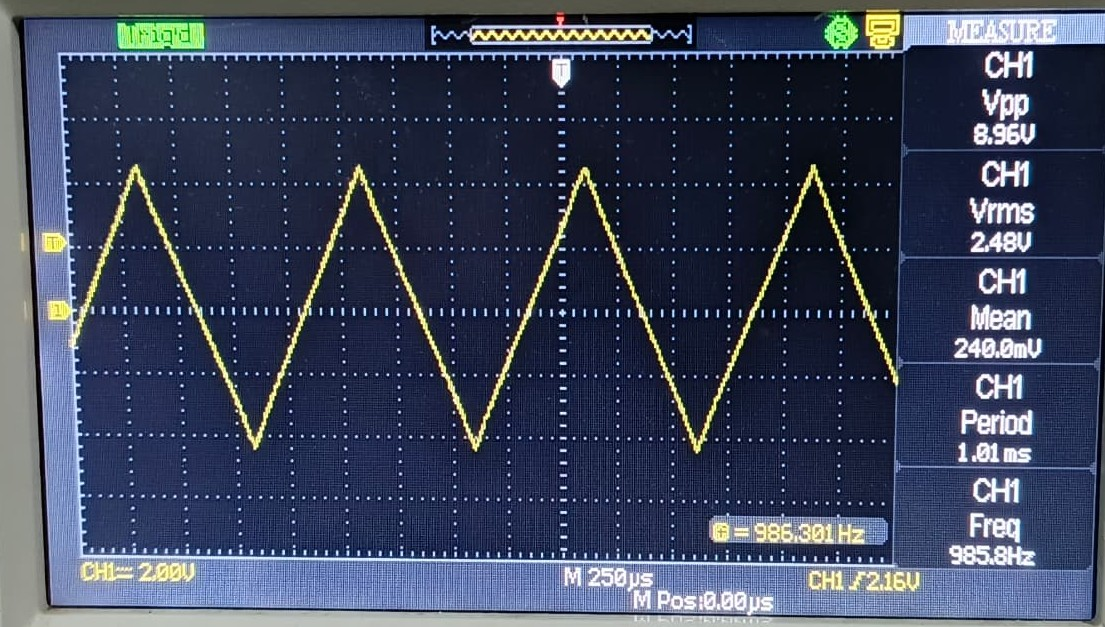
\includegraphics[width=\textwidth, keepaspectratio]{lab-05/assets/clipper/input-triangular-wave.jpeg}
    \caption{ }
  \end{subfigure}
  \hfill
  \begin{subfigure}[b]{0.49\textwidth}
    \centering
    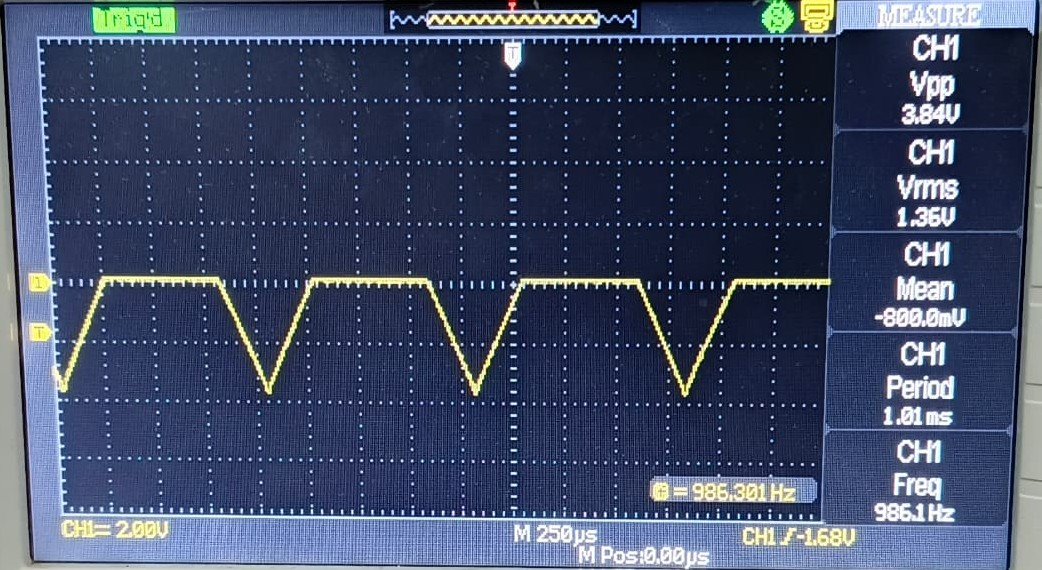
\includegraphics[width=\textwidth, keepaspectratio]{lab-05/assets/clipper/postive-output-triangular-wave.jpeg}
    \caption{ }
  \end{subfigure}

  \caption{(a) Input and (b) Output Wave Shape for Positive Clipper (Triangular Waves)}
  \label{fig:lab05_positive_triangular}
\end{figure}


